% 2010 年山东卷文科第 22 题：椭圆、直线 l 与点 P。
% 来源 PDF：普通高考/2010/2010山东文.pdf，SHA-256 95a69b861a29ca594f9118c9643efcdfd04cae3c4f374ff9fa009f7ac99712f4。
% 原页：第 2 页（A3 三栏）第 3 栏上部，书页码 622。
% 重绘依据：椭圆 x^2/2+y^2=1，F1(-1,0)、F2(1,0)；l:x+y=2；
%   P(0.4,1.6) 在 l 上，PF1 交椭圆于 A、B，PF2 交椭圆于 C、D。
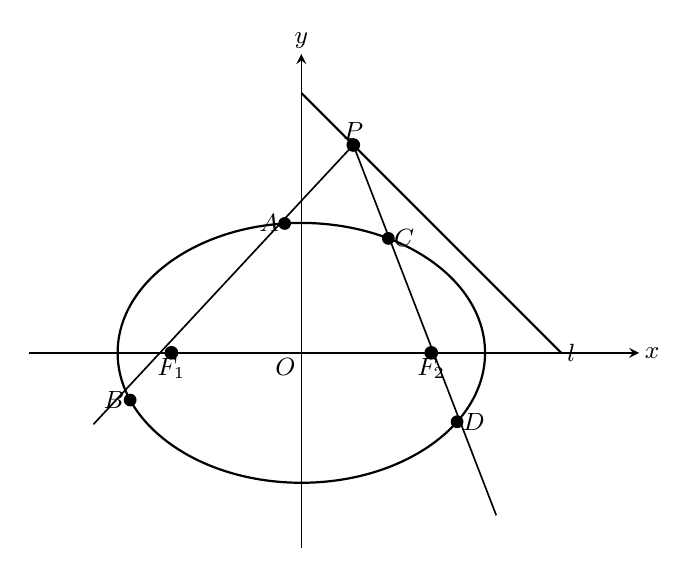
\begin{tikzpicture}[semithick, scale=1.65, every node/.style={inner sep=1.8pt, font=\small}]
  \draw[-stealth] (-2.1,0) -- (2.6,0) node[right] {$x$};
  \draw[-stealth] (0,-1.5) -- (0,2.3) node[above] {$y$};
  \draw[thick] (0,0) ellipse (1.414 and 1);
  \draw[thick] (0,2) -- (2,0) node[right] {$l$};
  \fill (-1,0) circle (1.5pt) node[below] {$F_1$};
  \fill (1,0) circle (1.5pt) node[below] {$F_2$};
  \fill (0.4,1.6) circle (1.5pt) node[above] {$P$};
  \draw (0.4,1.6) -- (-1.6,-0.55);
  \draw (0.4,1.6) -- (1.5,-1.25);
  \fill (-0.1286,0.9959) circle (1.4pt) node[left] {$A$};
  \fill (-1.3177,-0.3631) circle (1.4pt) node[left] {$B$};
  \fill (0.6697,0.8808) circle (1.4pt) node[right] {$C$};
  \fill (1.1989,-0.5304) circle (1.4pt) node[right] {$D$};
  \node[below left] at (0,0) {$O$};
\end{tikzpicture}
